\documentclass[a4paper,10pt]{article}
\usepackage{geometry}
\geometry{
  left=1cm,
  right=1cm,
  top=2cm,
  bottom=2cm,
  bindingoffset=5mm
}
\usepackage[ngerman]{babel}
\usepackage[utf8]{inputenc}
\usepackage{fancyhdr}
\usepackage{pdfpages}
\usepackage{parskip}

\usepackage[backend=biber,
style=alphabetic,]
{biblatex}

\addbibresource{library.bib}

\pagestyle{fancy}
\fancyhf{}
\rhead{AD Hausarbeit}
\lhead{Kristoffer Schaaf}
\rfoot{Page \thepage}

\newcommand*{\quelle}{%
  \footnotesize Quelle:
}

\title{BITS3-AD WS2021, Hausarbeit}
\author{Kristoffer Schaaf (2588265)} 

\begin{document}
\maketitle
\tableofcontents

\section{Einleitung}

\subsection{Aufgabenstellung}

Im Rahmen dieser Arbeit wird die Implementierung einer abstrakten Datenstruktur für eine Client/Server Anwendung (siehe Abbildung \ref{fig:nachrichtendienst}) behandelt. 

Die Aufgabe dieser Anwendung ist es Tagesnachrichten von verschiedenen Redakteuren zu verwalten und in korrekter Reihenfolge an den Kunden auszuliefern. Da die Reihenfolge der Nachrichten nicht von den Redakteuren abgestimmt wird, würde diese ohne einen Zwischenserver nicht korrekt sein. Die Nachrichten werden von dem Redakteur-Client-Programm mit einer eindeutigen Nummerierung zuerst an einen Server gesendet. Dieser wird über das abstrakte Datenstruktur-Konzept einer \textit{Holdback} und \textit{Delivery Queue} verwaltet. Das heißt, dass zuerst alle Nachrichten in der \textit{Holdback Queue} gehalten und nur bei korrekter Nummer an die \textit{Delivery Queue} weitergegeben werden.\\ 
Von der \textit{Delivery Queue} aus werden die Nachrichten auf Anfrage des Lesers dann in korrekter Reihenfolge an das entsprechende Client-Programm geschickt.\\

\begin{figure}[htbp]
\begin{center}
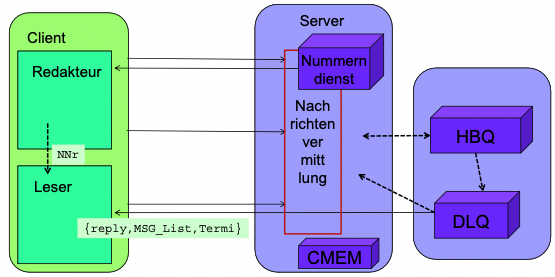
\includegraphics[scale=0.6]{Bilder/NachrichtendienstAbb.png}
\caption{\label{fig:nachrichtendienst} Nachrichtendienst \cite{Klauck2021}} 
\end{center}
\end{figure}

Da es auch hier wieder verschiedene Leser gibt hat der Server die Aufgabe sich für jeden Leser, insofern dieser sich nicht zu lange nicht mehr gemeldet hat, zu merken, welche Nachrichten er schon an diesen verschickt hat. 
Um den korrekten Ablauf der Anwendung kontrollieren zu können und um beim Implementieren Fehler möglichst einfach eliminieren zu können, werden alle Ausgaben in einer Datei \textit{HB-DLQ$<$Node$>$.log} geschrieben. Der Node auf welchem das System gerade läuft kann über den Erlang Befehl \textit{inet:gethostname()} bestimmt werden.

Da die beiden Client Programme für die Redakteure und Leser und der Server zur Verfügung gestellt wurden, wird es im folgenden um die Implementierungen der \textit{Holdback} und der \textit{Delivery Queue} gehen. Diese wird komplett in der funktionalen Programmiersprache Erlang umgesetzt.

\subsection{Funktion der Holdback Queue}

Die \textit{Holdback Queue} enthält alle Nachrichten, die nicht ausgeliefert werden dürfen. Das heißt, dass die enthaltenen Nachrichten nicht die richtigen Nummern für die \textit{Delivery Queue} haben. Durch regelmäßiges Prüfen wird entschieden, ob inzwischen eine geeignete Nachricht für die \textit{Delivery Queue} vom Server empfangen wurde. 

Da die Nachrichten nach aufsteigender Nummerierung an die \textit{Delivery Queue} weitergeleitet werden, bietet es sich an diese in der \textit{Holdback Queue} bereits zu sortieren. 
Um diese Sortierung möglichst effizient zu gestalten werden verschiedene Algorithmen getestet (siehe Kapitel \ref{Problemstellungen}.).

\subsection{Funktion der Delivery Queue}

Die \textit{Delivery Queue} ist der abstrakte Speicher für alle Nachrichten, welche an den Client ausgeliefert werden können. Die Nachrichten sind innerhalb der Queue aufsteigend sortiert. Die eigentliche Schnittstelle zum Server ist die \textit{Holdback Queue}, über diese werden die Nachrichten wieder versendet. Die \textit{Delivery Queue} ist somit lokal implementiert und wird von der \textit{Holdback Queue} aufgerufen. 

\subsection{Aufbau der Nachrichten}

Nachrichten werden von den Redakteuren entwickelt und von den Lesern konsumiert. Bis sie beim Leser ankommen, können sie aber durch mögliche Software Fehler, wie z.B. asynchrone Nebenläufigkeiten oder ähnliches, verloren gehen.\\
Die Nachrichten sind Tupel mit mindestens drei Elementen. Zum einen enthalten sie die Nachrichten-Nummer, nach welcher die Nachrichten sortiert werden. Zum anderen enthalten sie eine Textzeile in welcher die eigentliche Nachricht geschrieben steht. Abhängig davon, welche Queues sie schon durchlaufen haben, enthalten sie Zeitstempel mit den entsprechenden Eintritts- und Austrittszeiten. 

\subsection{Aufgabenerarbeitung}

Im Folgenden werden zuerst Entwürfe für die verschiedenen Queues mit ihren Funktionen erstellt, dabei wird vorerst nur die Implementierung der \textit{Holdback Queue} als Heap und die \textit{Delivery Queue} als Liste beschrieben. Die Entwürfe sollen nahe am zu implementierenden Code liegen, damit Fehler schnell eliminiert werden können. Um den Code zu testen werden Eunit Tests aus der Library \textit{'eunit/include/eunit.hrl'} geschrieben. Diese werden für spezifische Fälle angewendet, welche aus den Diagrammen der Entwürfe entschlossen werden können. Alle Elemente werden bei passender Nummerierung sofort von der \textit{Holdback} zu der \textit{Delivery Queue} weitergeleitet.
Nachdem die erste Version mit der Heapstruktur innerhalb der \textit{Holdback Queue} funktioniert, wird eine zweite mit einer Listenstruktur implementiert.
\newpage
Diese beiden zu analysieren und zu vergleichen wird der Hauptbestandteil dieser Ausarbeitung sein\footnote{Zum Analysieren werden die Benchmarks von Matz Heitmüller genutzt.}.
Des Weiteren wird auch der Einfluss von Implementierungen mit \textit{Pattern Matching} zu welchen mit \textit{if-else Statements} verglichen. Die Messwerte Nach diesem Teil wird ein Fazit erstellt in welchem die Messergebnisse ausgewertet werden. 

\subsection{Sortierung der Nachrichten} \label{Problemstellungen}

Aufgabe dieser Hausarbeit wird das Sortieren der Nachrichten innerhalb der \textit{Holdback Queue} sein. Hierfür werden verschiedene Sortieralgorithmen getestet. Für die verschiedenen Algorithmen werden verschiedene abstrakte Datenstrukturen benötigt. So würde z.B. bei \textit{Insertion Sort} nur das Konzept der Liste, also das 'Aneinander-pipen' von Elementen, reichen. Bei einem \textit{Heap Sort} Algorithmus würde eine Heapstruktur verwendet werden müssen. Dieses Konzept basiert auf der Baumstruktur mit Wurzelknoten und Teilbäumen.\\
Hier als Beispiele drei Sortieralgorithmen (siehe Abbildung \ref{fig:sortAlgo}). Aufsteigend, absteigend und random, bezieht sich hierbei auf die Liste welche sortiert wurde.

\begin{figure}[htbp]
\begin{center}
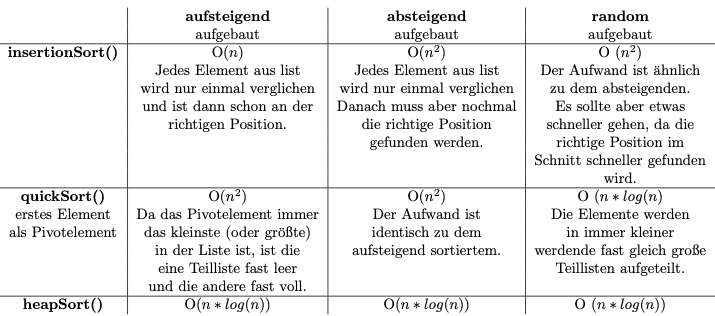
\includegraphics[scale=0.59]{Latex/Bilder/sortAlgo.png}
\caption{\label{fig:sortAlgo} Auswertung Sortieralgorithmen \cite{sortAlgo}} 
\end{center}
\end{figure}

Diese wurden bisher nur mit statischen Listen getestet. Hierbei wurde eine Liste übergeben, sortiert und der nächsten Prozess begonnen. In dieser Anwendung wird hierbei dynamisch gearbeitet. Da der \textit{Holdback Queue} frequent neue Nachrichten zugesendet werden, ist ein Algorithmus geeignet, welcher im Online-Verfahren arbeitet. Nicht alle zu sortierenden Elemente sind zu Beginn bekannt. Anbieten hierfür würde sich der \textit{InsertionSort} Algorithmus. 
Wie es der bereitgestellten logging Datei \textit{HB-DLQ@Qigong-KLC.log} (siehe Abbildung \ref{fig:HBQFilesEntry2}) zu entnehmen ist, werden die Nachrichten von den Redakteuren, mit zum größten Teil unbeständiger Nummerierung, gesendet. Für den \textit{InsertionSort} Algorithmus wäre dies aber ein Aufwand von O($n^2$).\\ Im Folgenden wird ein dem \textit{InsertionSort} ähnlicher Algorithmus verwendet. Im \textit{InsertionSort} sucht ein Laufindex das nächste unsortierte Element und fügt es an der richtigen Stelle in der Liste ein. In diesem Anwendungsfall wäre der Laufindex immer an der Position \textit{null}, da hier die neue Nachricht eingefügt wird. Der Index des Elements so lange erhöht, bis dieses die richtige Position erreicht hat. Wenn davon ausgegangen wird, dass die Elemente in zufälliger Reihenfolge eingefügt werden, entsteht eine Komplexität von $O(n/2)$. Beim Entfernen der Nachrichten gibt es in diesem Szenario den Vorteil, dass die Listen Erlang-Intern mit dem Listenkopf (Head) beginnen und an diese die restliche Liste (Tail) angehängt wird. Somit kann beim Entfernen des kleinsten Elements mit dem Tail weitergearbeitet werden, was auf einen Aufwand von $O(1)$ schließen lässt.

\begin{figure}[htbp]
\begin{center}
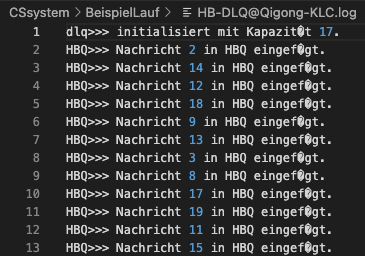
\includegraphics[scale=0.6]{Bilder/HBQFilesEntry.png}
\caption{\label{fig:HBQFilesEntry2} Nachrichtendienst \cite{HBQlogging}} 
\end{center}
\end{figure}

Der \textit{HeapSort} Algorithmus an sich setzt eine Komplexität von $O(n*log(n))$ voraus. Das liegt daran, dass die zu sortierende Liste zuerst zu einem Heap umstrukturiert werden muss. Man strukturiert den Heap in diesem Anwendungsfall von Anfang an, dadurch entfällt der Schritt. Es bleibt eine Komplexität von $O(log(n)$. Zu beachten ist, dass der Aufwand beim Einfügen und beim Entfernen auch beim Heap nicht identisch ist. Beim Einfügen gilt $O(log(n))$, da das Element eventuell nur den Heap nach oben wandert. Beim Entfernen gilt $O(2*log(n))$, da hier das Wurzelelement nach dem Entfernen ersetzt wird und der Heap somit auch neu strukturiert werden muss. Der \textit{HeapSort} Algorithmus ist bei aufsteigend sortierter Liste mit O($3*log(n)$) effizienter als der \textit{InsertionSort} Algorithmus. Mit gleichbleibender Effizienz aber deutlich besser bei random sortierter Liste. 

\subsection{Erwartungen} \label{erwartungen}

Das Ziel dieser Ausarbeitung ist es eine möglichst Effiziente Verarbeitung der Nachrichten zu erreichen. Der Fokus wird auf der Sortierung der Elemente innerhalb der \textit{Holdback Queue}, aber auch auf der Optimierung des allgemeinen Codes liegen.\\
Nach Vergleichen der beiden Implementierungen der \textit{Holdback Queue}, sollte die Sortierung über einen Heap als effizienter hervorgehen.\\
Außerdem wird geprüft, ob das Auslagern von Funktionen eine höhere Laufzeit zur Folge hat. Deswegen wird in einer Implementierung mit Hilfsfunktionen gearbeitet und in einer anderen auf diese verzichtet. Dies hat eine teilweise sehr tiefe Codestruktur und eine dementsprechend schlechte Lesbarkeit zur Folge. 


\section{Implementierung der Holdback Queue}

Wie bereits in Kapitel \ref{Problemstellungen} erläutert, wird die \textit{Holdback Queue} mit zwei verschiedenen Strukturen implementiert.

Für die Struktur des \textit{HeapSorts} gilt, dass jedes Element die Form \{$[$\textit{Nnr, Msg, TSclientout, TShbqin}$]$, Höhe, linkerTeilbaum, rechterTeilbaum\} hat. Außerdem ist die \textit{Nnr} des Wurzelelements stets kleiner, als die der Kinderelemente. Die beiden Kinderelemente werden nicht miteinander verglichen. Diese Form des Heaps nennt sich \textit{Min Heap} (siehe Abbildung. \ref{fig:binHeap}).

\begin{figure}[htbp]
\begin{center}
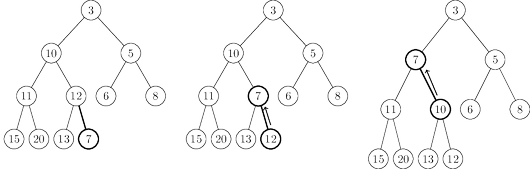
\includegraphics[scale=0.6]{Latex/Bilder/heapExample.png}
\caption[Binary Min Heap Insert]{Binary Min Heap Insert\footnotemark}\label{fig:binHeap} 
\end{center}
\end{figure}
\footnotetext{\url{https://rosalind.info/glossary/algo-binary-heap/}}

Für das Entfernen eines neuen Elements entsteht der Vorteil, dass das Element im Normalfall die Wurzel des Heaps ist, da es die kleinste Nachrichtennummer hat und somit ganz oben als Wurzel gespeichert ist. Beim Einfügen des Elements ist der Heap von Vorteil, da die Elemente ohne erkennbare Sortierung (siehe Abbildung \ref{fig:HBQFilesEntry}) vom Server in den Heap eingefügt werden. Die Elemente werden am höchsten freien Index eingefügt und wandern im Heap nach oben, bis sie ihre korrekte Position erreicht haben. Im Beispiel ist zu sehen, wie das Element mit der Nummer 7 eingefügt wird und solange mit dem Elternknoten getauscht wird, bis dieses größer ist. 

\begin{figure}[htbp]
\begin{center}
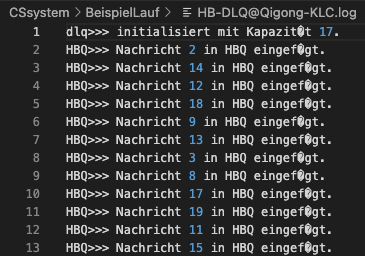
\includegraphics[scale=0.55]{Bilder/HBQFilesEntry.png}
\caption{\label{fig:HBQFilesEntry} Nachrichtendienst \cite{HBQlogging}} 
\end{center}
\end{figure}

Das Konzept des \textit{HeapSort} Algorithmus basiert darauf, dass die neuen Elemente als Blatt eingefügt und die sortierten Elemente als Wurzel entfernt werden. Im \textit{Min Heap} ist das Wurzelelement das kleinste Element des Baums. Dieser wird für die \textit{Holdback Queue} verwendet\footnote{Hierfür wurde der \textit{Max Heap} des zweiten Praktikums in Teilen wiederverwendet.}\footnote{Für weitere Informationen und Entwürfe über die Heap Funktionen siehe Anhang \ref{anhang} und \cite{sortAlgo}.}.

\subsection{initHBQ}

Das Initialisieren der \textit{Holdback Queue} wird durch die Erlang Funktion \textit{spawn/1}, an welche als Parameter die zu startende Funktion übergeben wird, realisiert. Hierbei wird ein neuer Prozess erzeugt und initialisiert. Die ProzessID dieses neu erzeugten Prozesses, wird als Rückgabeparameter in einer Variable gespeichert. 
Die globale Registrierung des Prozesses findet über den Aufruf \textit{register/2} statt. Als Parameter werden zum einen die ProzessID, des zu registrierenden Prozesses übergeben und zum anderen das Atom, unter welchem der Prozess gespeichert werden soll. 
Außerdem wird die Initialisierung der \textit{Delivery Queue} über die \textit{Holdback Queue} aufgerufen. Diesem Aufruf wird der Parameter DLQ-Limit, die maximale Größe der Delivery Queue, mit übergeben. 

Durch Rekursion kann der Status des Prozesses, unter anderem die Informationen über die \textit{Holdback} und \textit{Delivery Queue}, vollständig in den Parametern der Funktion gehalten werden (frei nach \cite{learnErlang}). Der Prozess der \textit{Holdback Queue} wird hierfür über die Funktion \textit{loop} gestartet. Dieser Funktion wird als Parameter die \textit{Holdback Queue} und dessen nächster freier Index oder Größe übergeben. Außerdem die \textit{Delivery Queue} mit maximaler Größe und die logging Datei. Somit können diese über jeden loop Aufruf beschrieben und gelesen werden. 
Ob der nächste freie Index oder die aktuelle Größe übergeben wird, hängt von der Struktur der \textit{Holdback Queue} ab. 

\subsection{checkHBQ} \label{checkHBQ}

Um die Nachrichten der \textit{Holdback Queue} regelmäßig auf Auslieferbarkeit zu prüfen, wurde hierfür eine weitere Funktion implementiert. 
In dieser wird das derzeitige erste Element der \textit{Holdback Queue} (im Folgenden 'SmallestElem') mit der von der \textit{Delivery Queue} erwarteten Nummer ('ExpNrDLQ') verglichen. 
Dadurch wird erkannt, ob Elemente aus der Holdback Queue verworfen oder an die Delivery Queue ausgeliefert werden sollen. 
Zum Beispiel wird im Fall SmallestElem == ExpNrDLQ das SmallestElem an die \textit{Delivery Queue} ausgeliefert. Bei SmallestElem $<$ ExpNrDLQ wird das SmallestElem verworfen, da es nicht mehr benötigt wird und die \textit{Holdback Queue} ansonsten blockieren würde. Benötigt wird es nicht mehr, da die Delivery Queue als aufsteigende Liste ohne Duplikate und ohne fehlende Nachrichtennummern definiert ist. Alle Nachrichten, welche eine kleinere Nachrichtennummer als das aktuell kleinste Element der \textit{Delivery Queue} haben, werden von dieser nicht mehr angefragt und können somit aus der Holdback Queue verworfen werden.  
Für den Fall, dass die Holdback Queue keine Elemente mehr enthält wird eine entsprechende Ausgabe geloggt. 

\begin{figure}[htbp]
\begin{center}
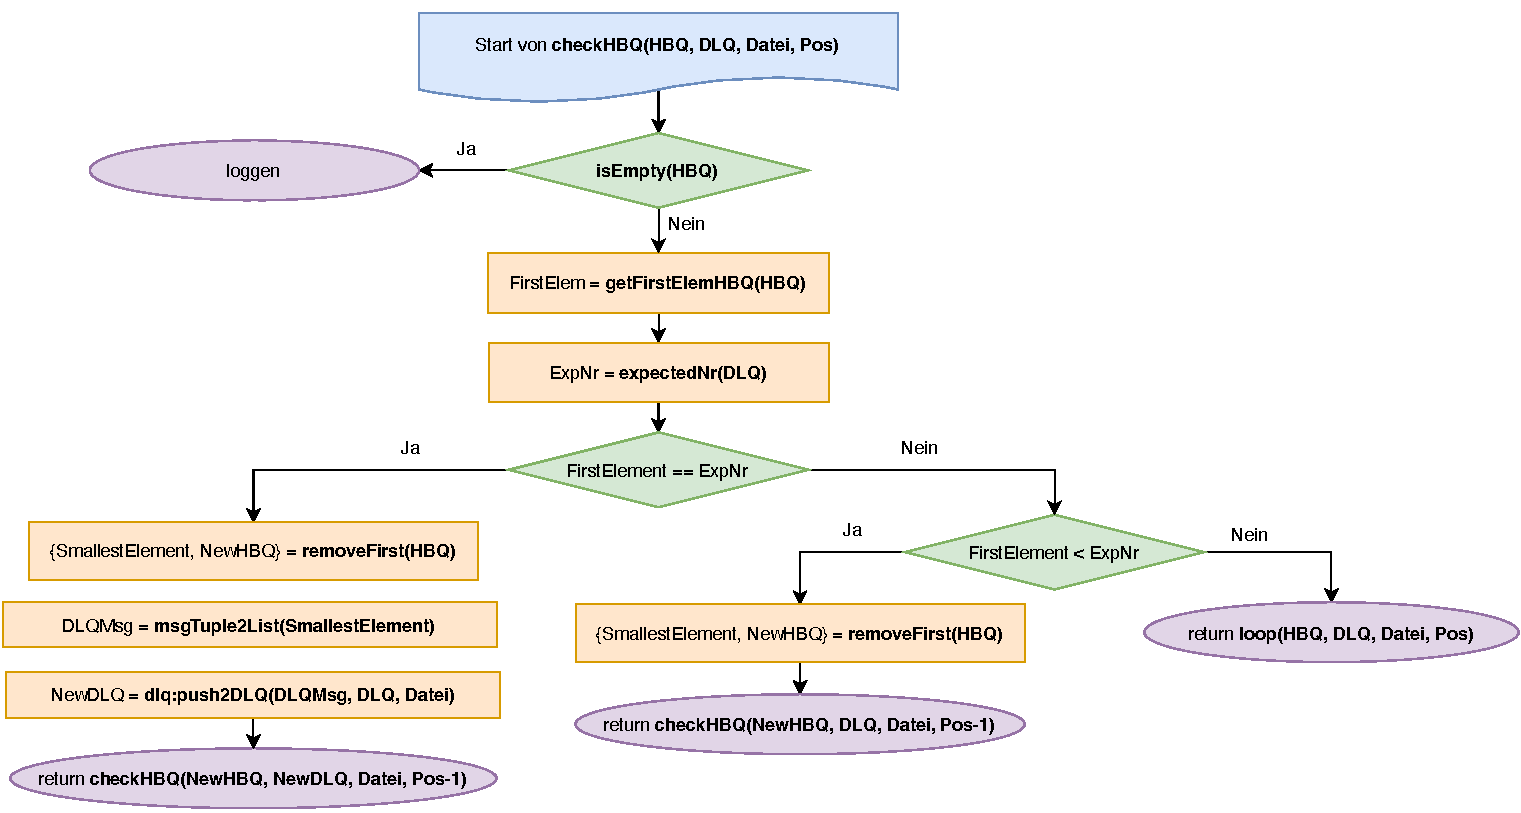
\includegraphics[scale=0.58]{Latex/Bilder/checkHBQ.pdf}
\caption{checkHBQ}\label{fig:checkHBQ}
\end{center}
\end{figure}

Wenn also zum Beispiel nur Elemente größer 3 in die \textit{Holdback Queue} eingefügt wurden, dann fehlen die Elemente 1, 2 und 3 zum Einfügen in die \textit{Delivery Queue}. In der Fehlermeldung steht "Fehlernachricht für Nachrichten 1 bis 3 generiert.". Die 3 wird als Nachricht zusätzlich in die \textit{Delivery Queue} eingefügt.

Die Funktion wird nach jeder Ausführung der \textit{pushHBQ} Funktion aufgerufen. Somit ist sichergestellt, dass nach jeder Veränderung der Queue einmal geprüft wird, ob diese noch synchronisiert ist und keine für die \textit{Delivery Queue} geeignete Nachricht vom Server geschickt wurde.

\subsection{pushHBQ} 

In dieser Funktion wird eine Nachricht in die \textit{Holdback Queue} geschrieben. Die Nachricht enthält die entsprechende Nachrichtennummer und den Inhalt der Nachricht. Außerdem einen Timestamp, wann der Client die Nachricht abgeschickt, bzw. die \textit{Holdback Queue} diese empfangen hat. 

Bedingt durch die fehlende Sortierung der Clients, wird jedes Element als Blatt eingefügt\footnote{Zum Bestimmen des Pfades der nächsten freien Blatts wird wie in der letzten Praktikumsaufgabe die sortv.erl Datei \cite{sortv} verwendet.}. Hier wird als Parameter die Position, also der höchste freie Index, mit übergeben. Dieser muss bei jedem Einfügen eines Elements erhöht und beim Löschen eines Elements um eins verkleinert werden. 

\begin{figure}[htbp]
\begin{center}
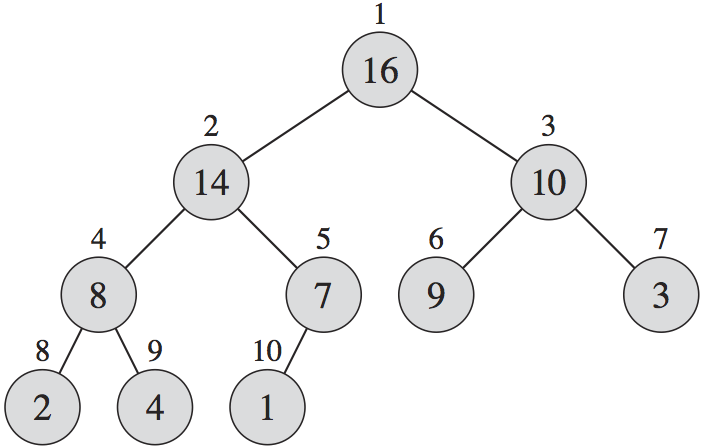
\includegraphics[scale=1]{Latex/Bilder/heapIndex.png}
\caption[Binary Heap Index]{Binary Heap Index\footnotemark}\label{fig:binHeapIndex}
\end{center}
\end{figure}
\footnotetext{\url{https://weibeld.net/algorithms/data-structures.html}}

\newpage

\begin{lstlisting}
% sortv.erl
% @author: Prof Dr Christoph Klauck, HAW Hamburg 
calcPath(Number) -> calcPath(Number,[]).
% aktuelle Position ist Wurzel
calcPath(1,Accu) -> Accu;
% aktuelle Position ist gerade
calcPath(Number,Accu) when Number rem 2 =:= 0 -> calcPath(Number div 2,[l|Accu]);
% aktuelle Position ist ungerade
calcPath(Number,Accu) when Number rem 2 =/= 0 -> calcPath((Number-1) div 2,[r|Accu]).	
\end{lstlisting}

Anhand dieses Indexes kann der Pfad durch modulo Rechnungen bestimmt werden. Wird wie im Beispiel in der Abbildung \ref{fig:binHeapIndex} eine ungerade Position, in diesem Fall die 11, übergeben, wird der Pfad \textit{$[l|r|r]$} zurückgegeben. Es müssen also zuerst der linke Teilbaum und dann zweimal der rechte Teilbaum gewählt werden, um in das nächste freie Blatt zu gelangen.
Die Position des höchsten Index wird als Integer zusammen mit der Holdback Queue als Parameter in der loop Funktion mit übergeben und somit rekursiv gespeichert. 

Bedingt durch die limitierte \textit{Delivery Queue} Größe, wird der Inhalt der \textit{Holdback Queue} ab einer erreichten Größe von $\frac{2}{3}*sizeOf(DLQ)$ reduziert. Dafür wird geprüft, wie groß die Lücke zwischen den beiden Queues ist. Ein Beispiel dafür ist in Abbildung \ref{fig:BeispielHBQFehler} zu sehen. Hier hat die \textit{Holdback Queue} diese bestimmte Größe erreicht und die Lücke in der \textit{Delivery Queue} wird dementsprechend aufgefüllt. Aufgefüllt werden hierbei nicht alle fehlenden Nachrichten, sondern nur die von der \textit{Delivery Queue} zuletzt erwartete. Eine ähnliche Fehlermeldung wie in der Abbildung wird in Textform in diese Nachricht als \textit{Msg} eingetragen. 

\begin{figure}[htbp]
\begin{center}
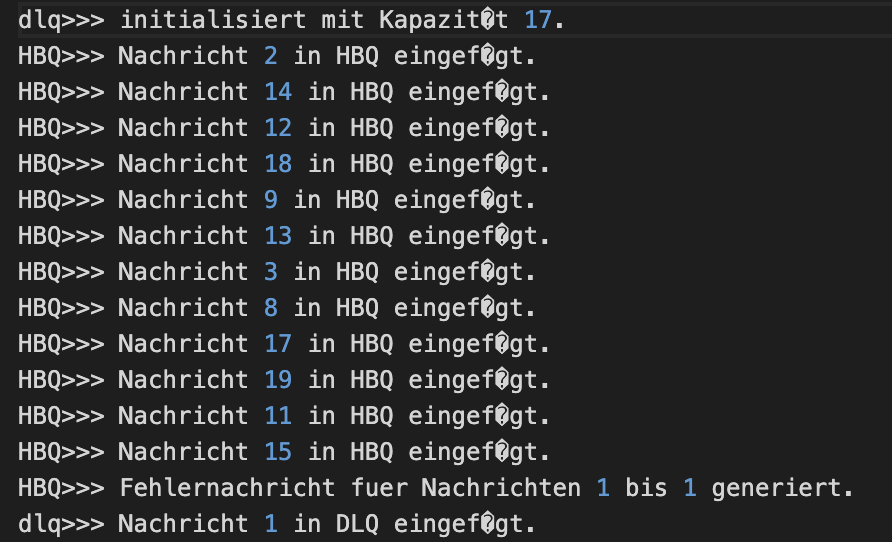
\includegraphics[scale=0.6]{Bilder/BeispielHBQFehler}
\caption{\label{fig:BeispielHBQFehler} Fehlermeldung Beispiel \cite{HBQfehler}} 
\end{center}
\end{figure}

Die Elemente, welche aus der \textit{Holdback Queue} an die \textit{Delivery Queue} gesendet wurden, werden aus der \textit{Holdback Queue} gelöscht, da ansonsten die Größe der Queue nicht aktualisiert werden kann. 

Ein weiteres Problem entsteht, wenn Elemente eingefügt werden, welche eine kleinere Nachrichtennummer haben als das zu erwartende nächste Element der \textit{Delivery Queue}. \\
In diesem Falle wird die einzufügenden Nachricht verworfen und es wird NNr<expNrDLQ an den Prozess gesendet, welcher in der \textit{Holdback Queue} gespeichert ist.

\subsection{deliverMSG}

In dieser Funktion wird die \textit{Delivery Queue} über die \textit{Holdback Queue} beauftragt die zu der übergebenen Nachrichtennummer zugehörige Nachricht zu senden. Der Client welcher die Nachricht empfangen soll wird als ProzessID mit im Parameter der Funktion übergeben. 
Über den Funktionsaufruf \textit{dlq:deliverMSG(MSGNr, ClientPID, Queue, Datei)} wird also die entsprechend zu sendende Nachrichtennummer, die ProzessID, die Delivery Queue und die in die zu loggende Datei übergeben. 
Wenn die übergebene Nachricht nicht verfügbar ist, dann wird die Nachricht mit der nächst größeren Nummer gesendet. 
Als Antwort sendet der Prozess der\textit{ Holdback Queue} die gesendete Nachrichtennummer. 

\subsection{listADT}

Diese Funktion ist aufgeteilt in zwei Funktionen: \textit{listHBQ} und \textit{listDLQ}. 
Es wird in beiden der Inhalt der jeweiligen Queue ausgegeben. Dabei wird die Reihenfolge der Queue beibehalten. Ausgegeben werden alle enthaltenden Nachrichtennummern in Form einer Liste. 

\paragraph{listHBQ}
Für diese Funktion wird über alle Elemente der \textit{Holdback Queue} iteriert und jeweils die Nachrichtennummer in eine separate Liste geschrieben. 
Da die \textit{Holdback Queue} in einer Heap Struktur umgesetzt ist, gibt es zwei mögliche Sortierungen. Zum einen könnte nach Index sortiert werden. Dementsprechend würde das Wurzelelement als erstes ausgegeben werden, dann alle Elemente mit der nächst kleinsten Höhe von links nach rechts gelesen usw..
Die andere Möglichkeit wäre es den Heap bei der Ausgabe zu sortieren. Dafür wird das Wurzelelement als erstes ausgegeben werden, vor der nächsten Ausgabe wird dann erst der Heap neu strukturiert. Das Element mit dem höchsten Index wird die neue Wurzel. Dieses versickert so lange nach unten, bis es keinen kleineren Teilbaum mehr hat. Erst danach wird das nächste Element (also wieder die Wurzel) ausgegeben. 
Der Vorteil der Index-Sortierung ist die kleinere Laufzeit, da im Vergleich zur Nachrichtennummer-Sortierung nicht nach jeder Ausgabe neu strukturiert werden muss. Allerdings sind bei der Index-Sortierung die Nachrichtennummern in der Ausgabe zufällig, was zum Beispiel das händische Finden eines Elements aufwändiger macht. 
Da die Funktionalität in diesem Falle im Vordergrund steht, wird bei \textit{listHBQ} eine Liste in aufsteigend sortierter Reihenfolge ausgegeben. 

Die Ergebnisse werden in eine log Datei geschrieben und bei Erfolg wird als Rückgabewert \textit{ok} als Antwort gesendet.

\paragraph{listDLQ}
Die bereits existierende Funktion \textit{listDLQ} der Delivery Queue, wird hier verwendet. 
Als Queue wird die in der \textit{Holdback Queue} gespeicherte \textit{Delivery Queue} übergeben und die zurückgegebene Liste wird dann in die Logging Datei geschrieben. 

\subsection{dellHBQ}

Um die \textit{Holdback Queue} zu löschen, muss durch die rekursive Implementierung die Funktion loop/4 beendet werden. Dadurch, dass diese Funktion als Schleife implementiert ist, wird durch den Funktionsaufruf \textit{dellHBQ} die Abbruchbedingung simuliert. Nach diesem Aufruf sind dann weder die Elemente innerhalb der Queue noch vorhanden, noch ist die Prozess ID der Queue weiterhin referenziert. 
Außerdem wird das Löschen der \textit{Delivery Queue} von dieser Funktion initialisiert. 



\section{Implementierung der Delivery Queue} \label{dlq}

Die \textit{Delivery Queue} enthält alle Nachrichten, die an den Leser ausgeliefert werden dürfen. Sie hat einen begrenzten Speicher zur Verfügung, welcher nicht überschritten werden darf. Dieser wird bei Initialisierung der Queue übergeben und innerhalb der Queue gespeichert. Die Nachrichten werden in der \textit{Delivery Queue} in einem \textit{First-In First-Out} Speicher abgelegt. Die Nachricht die als erstes eingefügt wird, verlässt dementsprechend als erstes wieder die Liste (siehe Abbildung \ref{fig:fifo}).

\begin{figure}[htbp]
\begin{center}
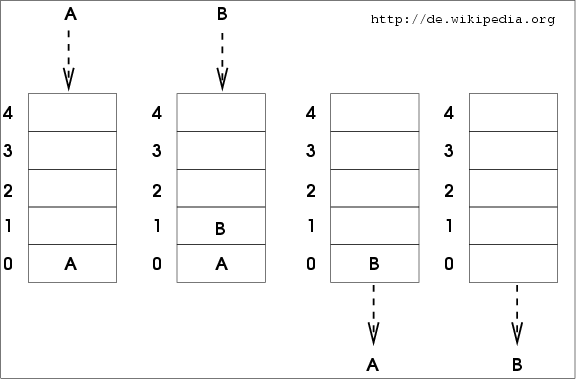
\includegraphics[scale=0.4]{Latex/Bilder/FIFO_PEPS.png}
\caption[First In First Out]{FIFO\footnotemark}\label{fig:fifo}
\end{center}
\end{figure}
\footnotetext{\url{https://de.wikipedia.org/wiki/First_In_–_First_Out}}

Dafür werden die neuen Elemente immer an die Liste angehängt, so dass die Nachricht mit der kleinsten Nummer immer an letzter Stelle eingefügt wird. Hierfür bietet sich in Erlang das Anfügen an. 

\begin{lstlisting}
NewDLQ = OldDLQ ++ [NewMessage]
\end{lstlisting}

In dieser Funktion werden zwei Listen zu einer kombiniert. Das zweite Element muss als Liste übergeben werden. Es ist mit der Struktur \textit{NewMessage = [NNr, Msg, TSclientout, TShbqin, TSdlqin]} zwar schon eine Liste, aber weil die Nachricht als ein Element eingefügt werden soll, muss es als Liste mit nur einem Element angefügt werden werden. 
Die Liste wird aufsteigend sortiert, da theoretisch genauso viele Elemente in die Liste eingefügt, wie auch wieder aus der Queue gelöscht werden. 

Ein Problem bei der \textit{Delivery Queue} stellt die vorgegebene maximale Größe dar. Diese kann nicht im Speicherplatz reserviert werden (keine In-Place Lösungen in Erlang), wie zum Beispiel über ein malloc in C oder über ein Attribut wie in Java. Die Größe muss im Prozess der Queue oder direkt in der Queue gespeichert werden.
Die erste Möglichkeit zur Speicherung der Größe bietet aber viele Fehlerquellen. Die Implementierung würde in Teilen wie folgt aussehen:
\begin{lstlisting}
spawn(fun() -> loop(Size, Datei, 0) end).

loop(MaxSize, Datei, ActSize) -> 
    receive 
        {From, getVariables} -> 
            From ! {reply, {MaxSize, Datei, ActSize}}
            loop(MaxSize, Datei, ActSize);
        {From, setVariables, {NewMaxSize, NewDatei, NewActSize}}
            From ! {reply, variablesSet}
            loop(NewMaxSize, NewDatei, NewActSize)
    end.
\end{lstlisting}

Über die Schnittstelle \textit{\{self(), getVariables\}} und \textit{\{self(), setVariables, \{NewMaxSize, NewDatei, NewActSize\}\}} können nun sowohl von der \textit{Holdback Queue} als auch von der \textit{Delivery Queue} aus das Limit der \textit{Delivery Queue}, die aktuelle Größe und die Logging Datei gelesen und geschrieben werden. Die \textit{Delivery Queue} wäre somit eine zum Teil entfernte abstrakte Datenstruktur. 
Ein Problem, welches nach der Implementierung entstanden ist, war das sehr aufwändige Debuggen von Fehlern oder Aufrufen innerhalb der Delivery Queue. 

Eine einfachere Lösung wäre das Speichern der Variablen innerhalb der Queue. 
Diese neue Queue hat die Struktur eines Tupels mit drei Elementen. Zum einen die maximale und die aktuelle Größe und zum anderen die eigentliche Queue in Form einer Liste - also \textit{DLQ = \{MaxSize, ActSize, [Msg1, Msg2, ...]\}}. So werden mögliche Fehler, welche durch Nebenläufigkeiten entstehen können, eliminiert. \\
Im Folgenden wird mit der zweiten Lösung, also der Speicherung der Elemente innerhalb der Delivery Queue als Tupel, gearbeitet.

\subsection{initDLQ}

In der Initalisierungfunktion der Delivery Queue wird die Queue erzeugt. Die Funktion hat den Aufruf \textit{initHBQ} und bekommt die maximale Größe und die Logging Datei mit übergeben. 
Nach erfolgreicher Initialisierung wird die Initialisierungsgröße der Delivery Queue geloggt und ein Tupel mit den Elementen \textit{MaxSize}, \textit{ActSize} und der eigentlichen Queue zurückgegeben.

\subsection{delDLQ}

Die \textit{Delivery Queue} wird in dieser Implementierung nicht als entfernte abstrakte Datenstruktur umgesetzt. Es muss dementsprechend kein Prozess beendet werden. Die Funktion gibt beim Aufruf \textit{ok} zurück.

\subsection{expectedNr}

Diese Funktion liefert die Nachrichtennummer die als nächstes in der \textit{Delivery Queue} gespeichert werden kann. Diese ist die größte enthaltene Nummer um eins erhöht. Die größte Nummer ist stets das letzte Element der Delivery Queue. Es wird rekursiv eine Teilliste der Queue aufgerufen und das erste Element dieser gespeichert, bis die Teilliste leer ist (siehe getLastElem/1). 
\begin{lstlisting} 
getLastElem([[NNr, _Msg, _TSclientout, _TShbqin, _TSdlqin]|[]]) -> NNr;
getLastElem([_Head|Tail]) -> getLastElem(Tail).
\end{lstlisting}

\subsection{push2DLQ}

Diese Funktion wird von der \textit{Holdback Queue} über die zugehörige Schnittstelle \textit{\{self(), \{request, pushHBQ, Msg\}\}} aufgerufen.

Die Funktion \textit{push2DLQ} speichert die übergebene Nachricht in der \textit{Delivery Queue}. Da die Queue bereits sortiert ist und das letzte Element in der Queue das Größte ist, wird das neue Element mit Zeitstempel an die Liste angefügt. 
Bei jedem Funktionsaufruf wird die maximale Größe mit der aktuellen Größe verglichen. Wenn die Delivery Queue die maximale Größe erreicht hat, dann wird beim Einfügen eines neuen Elements das Älteste gelöscht. Dies kann in Erlang sehr effizient umgesetzt werden. Durch die Aufteilung der Liste in Startelement und Restliste kann zum Löschen des ersten Elements einfach mit der Restliste weitergearbeitet werden. 

\begin{figure}[htbp]
\begin{center}
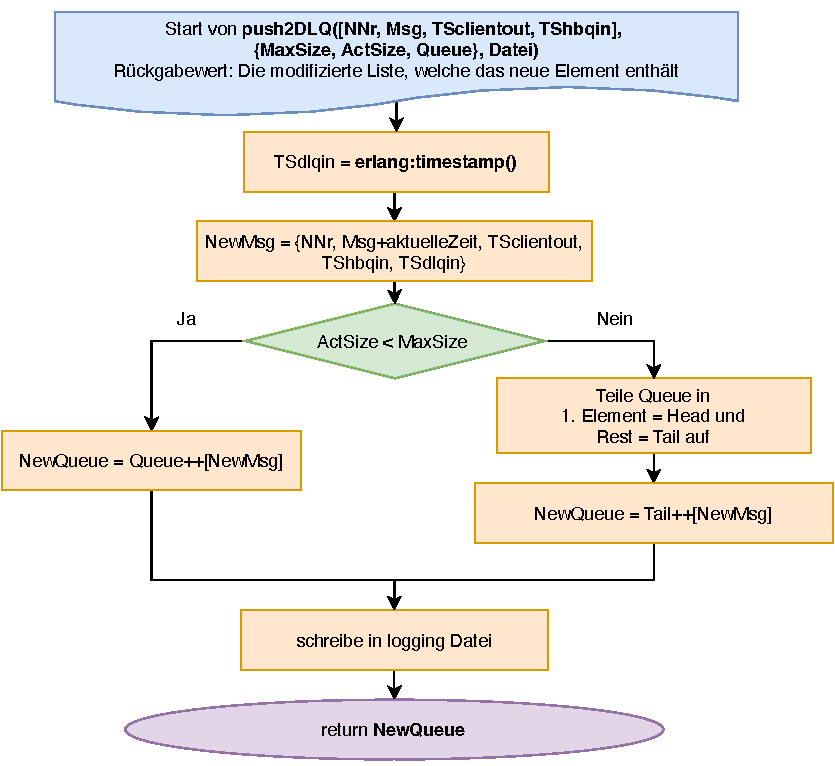
\includegraphics[scale=0.65]{Latex/Bilder/push2DLQ.pdf}
\caption{pushDLQ}\label{fig:pushDLQ}
\end{center}
\end{figure}

\subsection{deliverMSG}

Diese Funktion sendet die im Parameter übergebene Nachrichtennummer an die übergebene Prozess ID des Clients. Dafür wird durch die Elemente der Delivery Queue gelaufen, bis das Element entweder gefunden wurde oder das übergebene Element größer ist. 

\begin{lstlisting}
getMSGAtMSGNr(_MSGNr, []) -> [-1,nokb,0,0,0];
getMSGAtMSGNr(MSGNr, [[NNr, Msg, TSclientout, TShbqin, TSdlqin]|_Tail]) when MSGNr =< NNr-> 
    [NNr, Msg, TSclientout, TShbqin, TSdlqin];
getMSGAtMSGNr(MSGNr, [_Head|Tail]) -> getMSGAtMSGNr(MSGNr, Tail).
\end{lstlisting}

In obiger Funktion ist das rekursive Durchlaufen der Liste gezeigt. Der Funktion wird eine Liste übergeben, in diesem Falle die \textit{Delivery Queue}. Daraufhin wird von dieser Liste so oft das erste Element abgeschnitten, bis eine der beiden Abbruchbedingungen eintreffen. Anhand von \textit{Pattern Matching} kann verglichen werden, ob die Liste leer ist oder ob die erste Nachricht der übergebenen Liste größer gleich der gesuchten Nachrichtennummer ist.
Gelöscht werden die Elemente aus der Delivery Queue allerdings erst, sobald diese ihre maximale Größe erreicht hat.
Das eigentliche Senden der Nachricht an den Clienten findet innerhalb der Delivery Queue statt. \\Der Aufruf hat den Aufbau:
\textit{ClientPID ! \{reply,SendMessage,Terminated\}}

Um den gesamten Prozess terminieren zu können, wird der Delivery Queue von der Holdback Queue mitgeteilt ob diese noch Elemente enthält. Wenn das nicht mehr der Fall ist wird die Nachricht \textit{[-1,nkob,0,0,0]} mit einem weiteren Parameter \textit{true} übergeben.

\subsection{listDLQ}

Die Funktion gibt eine Liste mit den Nummern der in der \textit{Delivery Queue} enthaltenden Nachrichten zurück. Diese Nummern sind nach aufsteigender Größe sortiert, da am Kopf der Queue angefangen wird. Die Reihenfolge der Liste ist eingehalten. 

\subsection{lengthDLQ}

Diese Funktion gibt die Anzahl der in der \textit{Delivery Queue} enthaltenden Nachrichten zurück. Dafür wird die im Tupel der \textit{Delivery Queue} enthaltende Variable \textit{ActSize} zurückgegeben. 

\section{Problemstellungen} \label{Problemstellungen}

Problemstellung dieser Hausarbeit werden unter anderem das Testen verschiedener Datenstrukturen für die Holdback Queue sein. Da in dieser Queue eine Sortierung der Nachrichten stattfinden muss, bietet es sich an verschiedene Sortieralgorithmen zu testen und zu vergleichen. Für verschiedene Algorithmen werden dann aber auch dementsprechend verschiedene abstrakte Datenstrukturen benötigt. So würde z.B. bei Insertion Sort nur das Konzept der Liste, also das "Aneinander-pipen" von Elementen, reichen. Bei einem Heap Sort Algorithmus würde aber, wie der Name es schon andeutet, eine Heapstruktur verwendet werden müssen. Dieses Konzept basiert auf der Baumstruktur, es gibt also einen Wurzelknoten welcher einen linken und einen rechten Teilbaum haben kann. 

//TODO:
Die bisherigen Algorithmen wurden bisher nur getestet, wenn mit statischen Listen gearbeitet wurde. Es also eine Liste übergeben wurde, diese fertig sortiert wird und dann mit dem nächsten Prozess begonnen wird. In dieser Anwendung wird allerdings dynamisch gearbeitet. Da der Holdback Queue ständig neue Nachrichten zugesendet werden, wäre ein Algorithmus geeignet, welcher im Online-Verfahren arbeitet. Er kennt also nicht alle Elemente welche zu sortieren sind, wenn er mit dem Sortieren beginnt. Interessant hierfür wäre also der InsertionSort Algorithmus. 
Wie es der bereitgestellten logging Datei "HB-DLQ@Qigong-KLC.log" (siehe Abb. \ref{fig:HBQFilesEntry2}) zu entnehmen ist, werden die Nachrichten von den Client-Servern der Redakteure mit sehr unbeständiger Nummerierung gesendet. Für den InsertionSort Algoithmus wäre dies aber leider ein Aufwand von O($n^2$). 

\begin{figure}[htbp]
\begin{center}
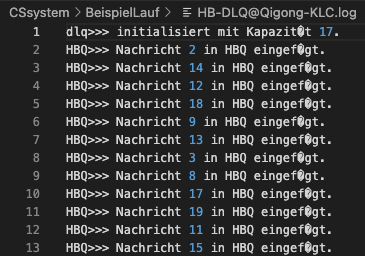
\includegraphics[scale=0.6]{Bilder/HBQFilesEntry.png}
\caption{\label{fig:HBQFilesEntry2} Nachrichtendienst \cite{HBQlogging}} 
\end{center}
\end{figure}

//TODO: Fragestellungen
Kann der Algorithmus sortieren während er die passenden Nachrichten an die Delivery-Queue ausliefert?

\section{Quellenverzeichnis}

\printbibliography

\end{document}